\section{Example}

In this chapter both approaches should be demonstrated within the example of the movie management software.  

\subsection{Automatic Test Generation: A Use Case Driven Approach}

In the first step the test objectives have to be derived. Therefore we define the use cases (can be thought of as main functions) and their contracts (\autoref{contracts1}) as requirement-level logical expressions. The contracts are used to infer the correct partial ordering of functionalities that the system should offer. Only the use cases that really impact the state of the transition system were specified for this example. The notation used is equal to the one proposed in the paper. 

\begin{lstlisting}[caption={Contracts attached to use cases},label={contracts1}]

UC createMovie(m: movie)
post createdMovie(m)

UC createLinkedPerformer(p: performer, m: movie)
pre createdMovie(m)
post createdPerformer(p) and createdLink(p,m)

UC rateMovie(m: movie)
pre createdMovie(m)
post calculatedOverallRating(m)

UC ratePerformer(p: performer)
pre createdPerformer(p)
post forall(m: movie){ createdLink(p,m)@pre implies calculatedOverallRating(m) }

UC linkExistingMovie(m: movie, p: performer)
pre createdMovie(m) and createdPerformer(p)
post not createdLink(p,m)@pre implies (createdLink(p,m) and calculatedOverallRating(m))

UC linkExistingPerformer(m: movie, p: performer)
pre createdMovie(m) and createdPerformer(p)
post not createdLink(p,m)@pre implies (createdLink(p,m) and calculatedOverallRating(m))

UC unlinkMovie(m: movie, p: performer)
pre createdMovie(m) and createdPerformer(p) and createdLink(p,m)
post calculatedOverallRating(m) and not createdLink(p,m) and not exists(m2: movie){ createdLink(p,m2) }@pre implies not createdPerformer(p)

UC unlinkPerformer(m: movie, p: performer)
pre createdMovie(m) and createdPerformer(p) and createdLink(p,m)
post calculatedOverallRating(m) and not createdLink(p,m) and not exists(m2: movie){ createdLink(p,m2) }@pre implies not createdPerformer(p)

UC removeMovie(m: movie)
pre createdMovie(m)
post not createdMovie(m) and forall(p: performer){ not createdLink(p,m) } and not exist(m2: movie){ createdLink(p,m2) }@pre implies not createdPerformer(p)

UC removePerformer(p: performer)
pre createdPerformer(p)
post not createdPerformer(p) and forall(m: movie){ not createdLink(p,m) }
\end{lstlisting}

After that the UCSystem prototype/interpreter tool should build the UCTS (\autoref{ucts}) through exhaustive simulation. The pool of parameters was restricted to one movie and performer to avoid a combinatorical explosion for this example. To build instantiated use cases the set of formal parameters are replaces with all the possible combinations of their actual vales. In our case we use the most simple approach by just having one possible combination. Furthermore the predicate calculatedOverallRating is no longer considered. Note that only predicates that evaluate to true are listed in the states as in the original paper. 

\begin{figure}[h]
	\centering
	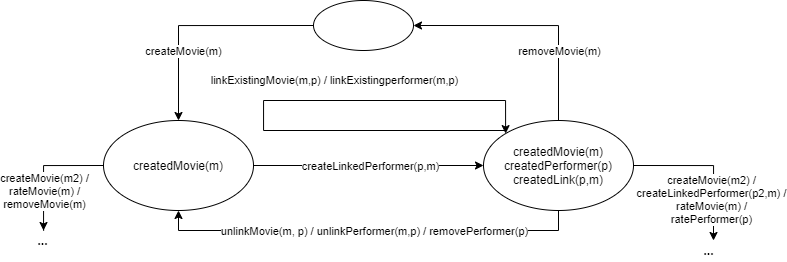
\includegraphics[width=1.0\textwidth]{img/ucts.png}
	\caption{The Use Case Transition System}
	\label{ucts}
\end{figure}

After applying an instantiated use case in the transition system (in case the precondition of the contract was fulfilled) the simulation state is updated according to the contracts' postcondition. 

Depending on the selected coverage criterion, we receive different test objectives as correct sequences of use cases. The robustness criterion was not considered in this example, but its application is coherent to the functional coverage criterions. How many test objectives are derived depends on the internal implementation of UCSystem and cannot be predicted for this example. Let's assume that one test objective is the test path createMovie(m) -> createLinkedPerformer(p,m) -> removeMovie(m). Then the use case scenarios from \autoref{ucs} are used to replace the use cases in the test objectives. It helps to specify the exchange of messages involved between the environment and the system.

\newpage

\begin{figure}[h]
	\centering
	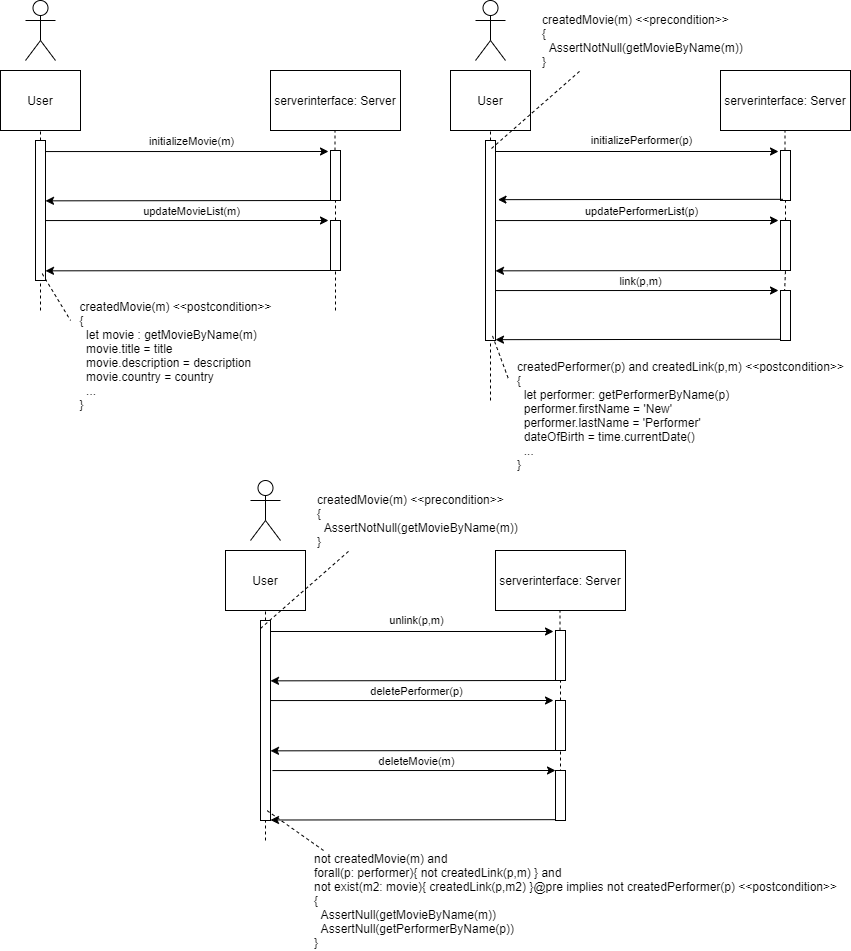
\includegraphics[width=0.65\textwidth]{img/ucs.png}
	\caption{The Use Case Scenarios}
	\label{ucs}
\end{figure}

Note that the use case scenarios may still be incomplete for the execution. They contain the main messages exchanged between the tester and the SUT and say how the system has to be simulated to perform a use case and how to react to the simulation. To know how the system has to be simulated, the use case scenarios contain more detailed contracts written in OCL besides the contracts written as logical expressions that were provided by the use cases. 

The UC-SCSystem uses the shown implementation in the use case scenarios to derive executable test scenarios as JUnit tests. 

\subsection{An Automated Approach to System Testing based on Scenarios and Operations Contracts}

The second approach differs from the first one as this time a transition system is built on a concrete use case, in our case the use case to unlink a movie from a performer. Input to the approach in this paper is the IOD (\autoref{iod}) with separate contracts defined in an OCL file (\autoref{contracts2}). IODs are a special form of activity diagrams used to show the control flow. The nodes in our case are UML sequence diagrams and define the operations of the contract transition system. The states are represented by the contracts themselves. 

\begin{figure}[h]
	\centering
	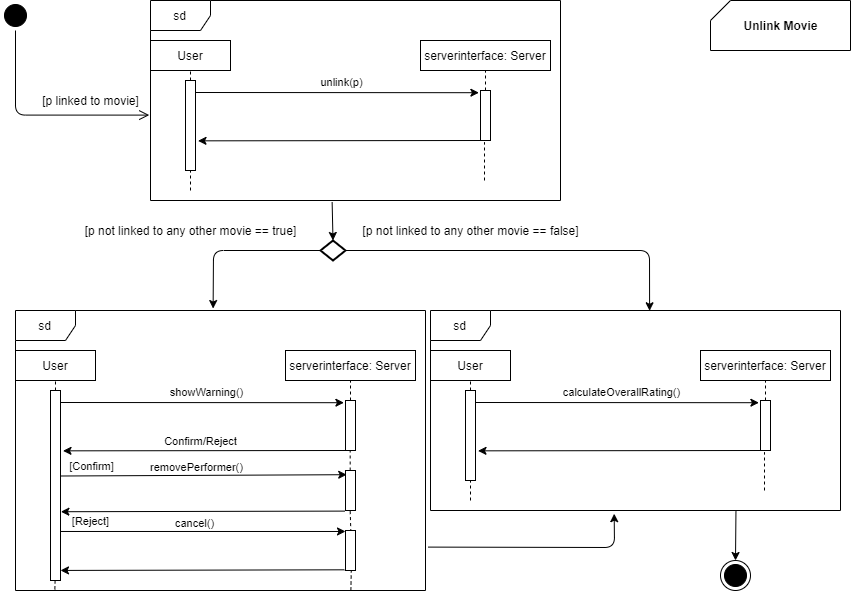
\includegraphics[width=\textwidth]{img/iod.png}
	\caption{Interaction Overview Diagram}
	\label{iod}
\end{figure}

\begin{lstlisting}[caption={Contracts written in OCL},label={contracts2}]
context Movie::unlink(performer)
pre  self.performers[performer] -> not isEmpty()
post self.performers[performer] -> isEmpty()

context MovieManager::removePerformer(performer)
pre forAll(movie | movie.performers[performer] -> isEmpty())
post self.performers[performer] -> isEmpty()

context Movie::calculateOverallRating()
post self.rating = 0.5 * (self.mean(self.performers.getRatings()) + self.rating)
\end{lstlisting}

\newpage

Based on the IOD and the specified contracts the CTS matrix gets defined and leads to the CTS shown in \autoref{cts}.

\begin{longtable}[h]{llll}
	Operations & Pre & Post & Composite States \\
	$O_{1}$ & $S_{0}$ & $S_{1}$ OR $S_{2}$ & A \\
	$O_{2}$ & $S_{1}$ & $S_{3}$ OR $S_{4}$ & B \\
	$O_{3}$ & $S_{3}$ OR $S_{4}$ & $S_{2}$ & \\
	$O_{4}$ & $S_{2}$ & $S_{5}$ & \\
\end{longtable}

\begin{figure}[h]
	\centering
	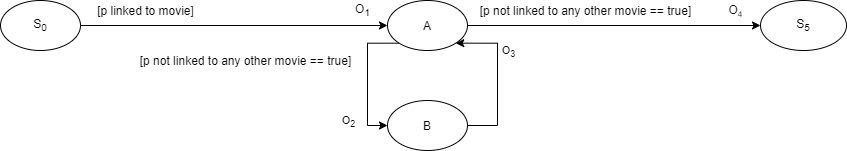
\includegraphics[width=\textwidth]{img/cts.png}
	\caption{Contracts Transition System}
	\label{cts}
\end{figure}

Based on a coverage criterion the test paths get derived. Differing from the first approach no test scenarios get generated. The paper shows a new more low-level approach to generate test paths as this was even a suggested improvement from the authors of the first paper. 
